The panel for this event application is as shown in
\autoref{fig:figure7}.  This application implements a scenario-based
(deterministic) seismic event.  In this panel the user specifies an
earthquake rupture (location, geometry and magnitude), a ground motion
prediction equation, a record selection database and the intensity
measure used for record selection.  In the backend, this application
relies on three other applications to perform seismic hazard analysis,
intensity measures simulation (to create a simulated target spectrum),
and ground motion record selection/scaling.  Users interested in
learning about those applications are referred to the documentation of
the
(\href{https://github.com/NHERI-SimCenter/GroundMotionUtilities/blob/master/Readme.md}{SimCenter
  ground motion utilities}).

\begin{figure}[!htbp]
  \centering {
    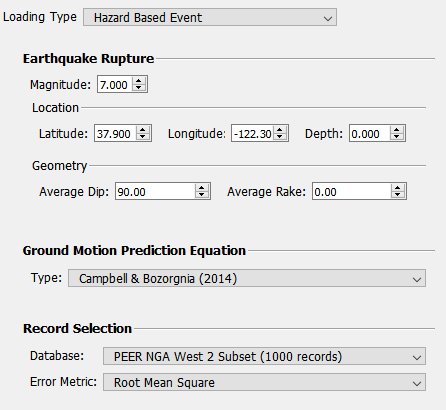
\includegraphics[width=0.8\textwidth]
    {usage/figures/hazardBased.png} }
  \caption{\texttt{Hazard Based Event} loading type}
  \label{fig:figure7}
\end{figure}
